\documentclass{article}
\usepackage[utf8]{inputenc}
\usepackage{biblatex}
\usepackage{amssymb}
\usepackage{amsmath}
\usepackage{marginnote}
\usepackage{hyperref}
\usepackage[shortlabels]{enumitem}
\usepackage{listings}
\usepackage{booktabs, multirow} % for borders and merged ranges
\usepackage{soul}% for underlines
\usepackage[table]{xcolor} % for cell colors
\usepackage{changepage,threeparttable} % for wide tables
\usepackage{graphicx,subfigure}
\usepackage{wrapfig}


\addbibresource{bib.bib}
\setlength{\parindent}{0em}
\bibliography{bib}


\title{Assignment 2}
\author{Atul Bipin, \textbf{abipin, 20648860}\\Zahin Mohammad, \textbf{z5mohamm, 20669584}}
\date{June 23, 2020}
\linespread{1.5}
\begin{document}

\maketitle
% \setlength{\parskip}{6pt}

% TODO: Describe different aspects (neighbor, etc.) of each question

% You	are	expected	to	turn	in	a	short	paper	(the	shorter	the	better)	which	should	
% include	the	following:
% 1)	A	short	description	of	your	program.
% 2)	A	description	of	your	implementation of	the	search	agent	with	memory	and	time	
% complexity	analysis.		
% 3)	Sample	output	of	your	program,	to	demonstrate	its	functioning

\section{Question 1}

\subsection{Program Description}

This is a \hl{simulated-annealing} program.
It is designed to find coordinates that lead to the global minimum of the $easom$ function.

\subsubsection{State Representation (Problem Formulation)}

The state of the program is represented as a vector $x$ (where $x = (x_1, x_2)^T$), signifying the location of the agent.
The agent's state is clipped to set bounds as described by,
\[x \in [-100,100]^2\]

The initial state here is picked randomly.

\subsubsection{Next Neighbor Function}

Given any state, the next neighbor is derived by randomly moving $x_1$ and $x_2$ to another part of the neighborhood (size of neighborhood is determined by Temperature ($T$)).
This process will be described in more detail in the "Implementaton" section below along with pseudo-code.

\subsubsection{Cost Function}

The cost of any given state is the value of the $easom$ function, described by:
\[f(x) = -cos(x_1)\,cos(x_2)\,e^{-(x_1 - \pi)^2 - (x_2 - \pi)^2}\]
where $x$ is:
\[x = (x_1, x_2)^T\]

\subsection{Implementaton \& Complexity}
The time-complexity for this algorithm is $O(n)$ where $n$ is the number of temperatures in the annealing schedule. The space complexity of simulated annealing is $O(1)$. It should be noted that our implementation is not strictly $O(1)$ as we store a list of states and costs for debug/print purposes, however these are not required. Additionally, the annealing schedule is made using a generator, therefore new iterations are lazily created.
\subsubsection{Simulated Annealing}

\begin{lstlisting}
    state = start_state
    initial_temp = get_initial_temperature()

    for T in annealing_schedule:
        cost = cost_function(state)

        new_state = neighbor(state, T, initial_temp)
        new_cost = cost_function(new_state)

        cost_diff = new_cost - cost

        if cost_diff <= 0:
            state = new_state
        else:
            prob = prob_of_acceptance(cost_diff, T)

            if prob > random():
                state = new_state

    return state
\end{lstlisting}

\subsubsection{Neighbor Function}

\begin{lstlisting}
    x1, x2 = x

    def move(xi):
        amplitude = (INTERVAL_SIZE) * (T/initial_temperature)
        # This negation ensures we can move up/down, left/right
        delta = (-amplitude / 2) + amplitude*random() 
        return xi + delta

    return move(x1), move(x2)
\end{lstlisting}
\subsubsection{Cost Function}
\begin{lstlisting}
    def cost_function(x1, x2):
        return -cos(x1) * cos(x2) * exp(-(x1-pi)**2 - (x2-pi)**2)
\end{lstlisting}

\subsection{Sample Output}
In the block of text below a sample output of the program can be viewed.
Figure \ref{fig:q1} shows the graphical comparison of the simulated annealing vs the actual search space.
\begin{lstlisting}
    Running Trigonometric Schedule
    Start State: (92.19460414241004, -29.695077749508414)
    Start Temp: 0.001
    Final State: (3.144010511144751, 3.143614114605061)
    Final Temp: 1e-05
    Iterations per T: 1000
    f(final_state): -0.9999851015970543
    Error from ideal value: 0.0014898402945662248%
\end{lstlisting}
\begin{figure}
    \centering
    {\label{fig:q1}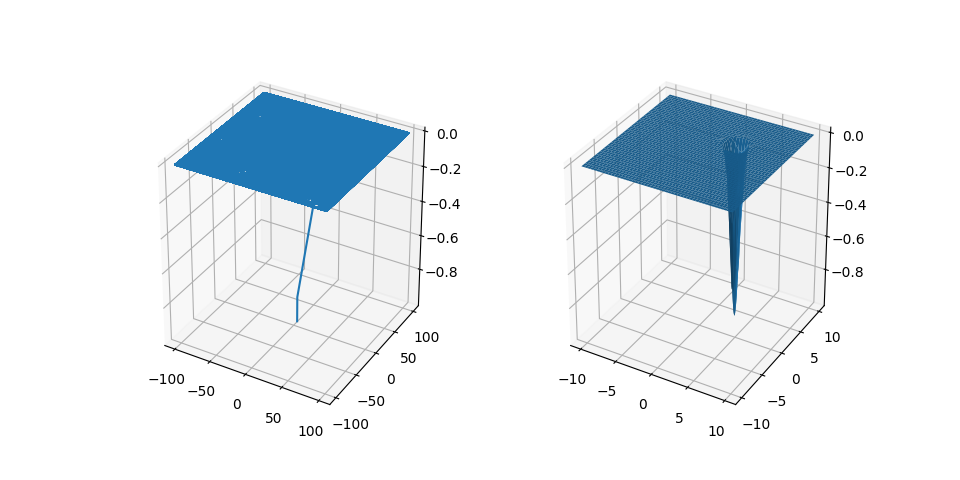
\includegraphics[scale=0.5]{q1.png}}
    \caption{Simulated Annealing vs Search Space}
\end{figure}

\newpage
\section{Question 2}

\subsection{Program Description}

This is a program designed to play the board-game "Conga".
The AI agent (part of the program) is designed to try and win the game in the least amount of moves possbible.
The AI agent uses \hl{minimax and $\alpha$-$\beta$ pruning} to make the best possible move with a search tree depth limit of 2.

\subsubsection{State Representation (Problem Formulation)}

The state of the program is represented as a 4x4 matrix, where the value of each cell in the matrix represents the amount of stones the corresponding player has.
The process of how white stones are differentiated from black stones will be discussed in the following section, "Implementation \& Complexity".
At any board configuration, an agent (AI or Random) can only move their own stones, and in a direction in which they are not blocked by the opponent agent.
Agent's cannot place stones outside of the defined 4x4 board matrix.

\setlength{\parskip}{6pt}

The initial state here is defined as per the rules of the game.
Player 1's stones are all located in (1,4), i.e. the top-left corner of the board and Player 2's stones are located at the opposite end (4,1).

\subsubsection{Next Neighbor Function}

The neighborhood for a given state $s$ is defined as all legal moves the agent can perform in that state. The legal moves are well-defined in the description of the game.

\subsubsection{State Evaluation Function}

The evaluation function, given state $s$, focuses on how many opponent stones are blocked against the board's walls or corner, and additionally the difference in cells controlled by the agent and the opponent.
The agent gives priority to the cost in the following order:

\begin{itemize}
    \item   {Blocks against a corner}
    \item   {Difference in controlled cells}
    \item   {Blocks against wall}
\end{itemize}

\subsection{Implementation \& Complexity}
The state is represented as an 4x4 matrx. All positive cells belong to white, and all negative cells belong to black. Cells marked as $0$ are free and belong to no one.

This time complexity for an AI agent to play against a random agent is $O(1)$. This is due to the fact that the game is stopping criterion where it will not play beyond 200 moves. If this stopping criterion was not in place the time complexity is unknown/not defined. Additionally, the program will do $minimax$ at each move which has a time complexity of $O(b^d)$ (with a best case of $O(b^{\frac{d}{2}})$ for $\alpha / \beta$ pruning) where $b$ is the branching factor and $d$ is the maximum depth. However depth is a known depth of $MAXDEPTH=2$, and additionally $b$ has a known constant upper-bound,  therefore the upper-bound for the $minimax$ algorithm is known to be a constant number. Lastly, the code deals with many serialize and de-serialize function calls for the board state, however the board is always a 4x4 matrix, therefore these are all $O(1)$ as well. Therefore, since any game played has an upper-bound defined for all operations, it is $O(1)$ time complexity.

This space complexity for an AI agent to play against a random agent is $O(1)$ ($O(d)$ but $d = MAX DEPTH$). All data-structures have a known upper-bound. Additionally, minimax is a memory-less algorithm so it does not store state information to memory.

\subsubsection{MiniMax function with A/B pruning}

\begin{lstlisting}
if depth == MAX_DEPTH or is_leaf_node(node):
    return evaluate(node)

if is_max:
    value = float('-inf')
    for child in get_children(node):
        value = max(value, minimax_dfs(
            child, False, depth + 1, alpha, beta))
        alpha = max(alpha, value)

        if alpha >= beta:
            break

    return value
else:
    value = float('inf')
    for child in get_children(node):
        value = min(value, minimax_dfs(
            child, True, depth + 1, alpha, beta))
        beta = min(beta, value)

        if beta <= alpha:
            break

return value
\end{lstlisting}

Minimax is used at the root node (which represents current state of the board) as follows:

\begin{lstlisting}
my_children_and_their_cost = []
my_alpha = float('-inf')
my_beta = float('inf')

children = get_children(root)

for child in children:
    child_cost = minimax_dfs(
        child, False, 1, my_alpha, my_beta)

    my_alpha = max(my_alpha, child_cost)

    my_children_and_their_cost.append(child_cost, child)

return my_children_and_their_cost
\end{lstlisting}

\subsubsection{Cost Function}

\begin{lstlisting}
for row in board:
    for col in row:
        if is_opponent(col):
            opponent_count += 1
        else:
            my_count += 1
        if is_opponent(col) and is_cornered(col):
            corner_count += 1
        else if is_opponents(col) and is_walled(col):
            wall_count += 1
return my_count - opponent_count + blocking_score(corner_count, wall_count)
\end{lstlisting}

\subsubsection{Neighbor Function}

\begin{lstlisting}
next_moves, next_move_costs = minimax(board)
best_moves = get_best_moves(next_moves, next_move_costs)
return random.choice(best_moves)
\end{lstlisting}

\subsection{Sample Output}

In Figure \ref{fig:q2} a sample output of the game is shown. Only the last few moves before the game is concluded is shown. If any user would like to see the full output, they will need to follow the instructions in the readme file for question 2. In the figure, the green-text player is the AI agent and the red-text player is the random agent.
\begin{figure}
    \centering
    {\label{fig:q2}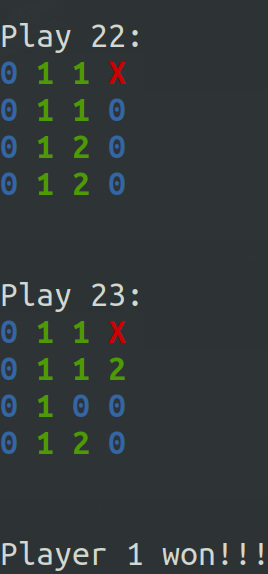
\includegraphics[scale=0.5]{q2.png}}
    \caption{AI agent vs Random agent in Conga}
\end{figure}

\newpage
\section{Question 3}

\subsection{Program Description}

This is a program that uses \hl{tabu-search} to search for an optimal placement of 20 departments into 20 locations that minimzes the costs between the placed departments.

\subsubsection{State Representation (Problem Formulation)}

The state $s$ is represented as an array of size 20.
The ordering of the elements in this array represents the placement of departments.

\setlength{\parskip}{6pt}

The initial state here was picked after testing 10 different random initial states/solutions and choosing the one that produced best results.
More details regarding this can be found below.

\subsubsection{Neighborhood Generation Function}

For a given state $s$, the neighborhood is generated by iteratively swapping two departments in the state array.
Each neighbor of state $s$ is one swap away from it.

\subsubsection{Cost Function}

The cost of a given state $s$ is computed as flow $*$ rectilinear distance between a pair of departments arranged as per the given state summed across all possible pairings.

\subsection{Implementation \& Complexity}

The time complexity of this implemntation of tabu-search is $O(1)$ as it has a stricht upper-bound on its iterating loop. Additionally the neighbor function is strichtly bounded by an upper-bound of 20, therfore it is $O(1)$. However, if the problem was generalized to support any size department planning, then the time complexity would change to $O(n)$ where $n$ is the number of departments. The stopping condition is a simple iteration counter that will stop when a certain user specified limit is reached.

The space complexity of this implementaiton of tabu-search is $O(m*n + j)$ where $m*n$ represent the size of the neighborhood in each iteration ($m$ is number of depertments and $n$ is the number of neighbors) and $j$ represents the size of the tabu-list.
\subsubsection{Tabu Search pseudo-code}

\begin{lstlisting}
s_best = initial_solution
best_score = evaluate(initial_solution)
current_solution = initial_solution
s_freq = {}
tabu_list = [initial_solution]

while not stopping_condition():
    # Increase freq penalty
    s_freq[current_solution] += 1

    neighborhood = get_neighbors(current_solution)

    if neighborhood is empty:
        end search

    if neighborhood only has tabu solutions:
        if no tabu solution is better than best solution so far:
            end search

    pick top candidate from neighborhood

    if top candidate is tabu and better than best solution:
        make it non-tabu
    else:
        pick another top candidate

    if non_tabu_top_score >= best_score:
        s_best = non_tabu_top_candidate
        best_score = non_tabu_top_score

    tabu_list.append(non_tabu_top_candidate)

    if len(tabu_list) > max_tabu_size:
        tabu_list.popleft()

    current_solution = top candidate
return s_best
\end{lstlisting}

The stopping condition (other than what's embedded into the tabu search) is just a specified number of max iterations.

\subsubsection{Solution Evaluation Function}
\begin{lstlisting}
sum = 0.0

for i from 0 to 19:
    for j from i+1 to 19:
        d_i, d_j = s[i], s[j]
        sum += flow[d_i, d_j] * distance[i, j]
        
return -sum - solution_frequency*2
\end{lstlisting}

A solution is evaluated to a negative value as the tabu search is maximizing in this case but we want to minimize the cost.

\subsubsection{Get Neighbor Function}

\begin{lstlisting}
initialize neighborhood to empty array
for i from 0 to 19:
    for j from i+1 to 19:
        neighbor = swap elements at i and j
        add neighbor to neighborhood

return neighborhood
\end{lstlisting}

\subsection{Sample Output}
The sample output for question-3 can be seen in the code block below.
\begin{lstlisting}
    Initial State: 15 6 11 7 10 5 0 13 16 18 9 14 17 2 12 19 3 8 4 1
    Initial Cost: 1750.0
    Final State: 8 2 9 13 17 15 10 11 1 3 12 7 19 14 18 5 0 6 4 16
    Final Cost: 1285.0
\end{lstlisting}

\subsection{Tabu Search Modifications}

Below are all the required tests as specified in the assignment.

\subsubsection{Change the initial starting point (initial solution) 10 times}

The output for 10 random inputs can be seen in the code block below.

\begin{lstlisting}
    Case 1:
    Initial State: 10 18 4 2 5 16 11 6 13 17 3 8 12 7 1 0 9 15 14 19
    Initial Cost: 1719.0
    Final State: 16 17 9 2 5 0 11 13 6 4 7 14 1 19 12 15 10 18 3 8
    Final Cost: 1346.0
    
    Case 2:
    Initial State: 13 7 18 8 3 5 6 4 19 14 15 9 2 12 16 17 10 0 11 1
    Initial Cost: 1773.0
    Final State: 17 1 18 3 16 2 9 14 0 4 8 13 11 6 5 15 10 7 19 12
    Final Cost: 1327.0
    
    Case 3:
    Initial State: 15 6 11 7 10 5 0 13 16 18 9 14 17 2 12 19 3 8 4 1
    Initial Cost: 1750.0
    Final State: 15 0 10 7 16 12 6 11 19 3 5 4 9 14 18 8 2 13 1 17
    Final Cost: 1292.0
    
    Case 4:
    Initial State: 3 9 4 2 6 16 8 1 12 13 7 18 14 17 15 0 10 11 5 19
    Initial Cost: 1708.0
    Final State: 16 6 4 5 12 3 19 18 1 17 7 11 14 13 2 10 0 15 9 8
    Final Cost: 1332.0
    
    Case 5:
    Initial State: 6 3 9 19 5 8 15 17 7 1 13 11 10 2 4 0 14 16 12 18
    Initial Cost: 1705.0
    Final State: 8 17 16 4 12 2 9 0 6 5 13 11 7 14 19 15 10 3 1 18
    Final Cost: 1325.0
    
    Case 6:
    Initial State: 9 11 2 4 5 19 3 0 14 12 17 15 1 13 18 16 7 8 10 6
    Initial Cost: 1708.0
    Final State: 4 6 0 5 12 7 19 11 9 2 18 14 1 13 8 16 3 10 17 15
    Final Cost: 1325.0
    
    Case 7:
    Initial State: 13 7 10 15 2 9 18 19 8 17 16 12 6 11 4 0 3 1 5 14
    Initial Cost: 1730.0
    Final State: 3 13 10 15 8 1 11 19 6 12 18 14 7 4 5 16 17 9 0 2
    Final Cost: 1301.0
    
    Case 8:
    Initial State: 8 9 17 2 0 4 18 15 11 14 16 12 10 7 1 13 3 5 6 19
    Initial Cost: 1615.0
    Final State: 2 9 18 17 16 8 13 1 14 11 15 10 3 7 0 12 5 4 19 6
    Final Cost: 1337.0
    
    Case 9:
    Initial State: 5 1 8 16 2 4 12 7 19 0 10 14 11 9 17 3 6 13 18 15
    Initial Cost: 1625.0
    Final State: 12 5 4 9 8 19 6 11 0 2 14 1 7 13 17 18 3 10 15 16
    Final Cost: 1316.0
    
    Case 10:
    Initial State: 1 4 3 9 14 0 17 13 2 5 8 6 11 10 15 7 12 18 16 19
    Initial Cost: 1787.0
    Final State: 16 0 17 2 5 3 4 18 9 12 10 6 19 1 15 7 11 14 13 8
    Final Cost: 1373.0
\end{lstlisting}

\subsubsection{Change the tabu list size: Static}

From the first random 10 cases, case 3's input was chosen for this test.
Below is the output of changing the tabu list size with a static value.
From the results it seems that a large tabu list size will degrade performance.
The lower bound test was too close to our initial value therefore no comments can be made on the lower bound.

\begin{lstlisting}
    Tabu List Size: 2
    Initial State: 15 6 11 7 10 5 0 13 16 18 9 14 17 2 12 19 3 8 4 1
    Initial Cost: 1750.0
    Final State: 8 2 9 13 17 15 10 11 1 3 12 7 19 14 18 5 0 6 4 16
    Final Cost: 1285.0
    
    Tabu List Size: 5
    Initial State: 15 6 11 7 10 5 0 13 16 18 9 14 17 2 12 19 3 8 4 1
    Initial Cost: 1750.0
    Final State: 8 2 9 13 17 15 10 11 1 3 12 7 19 14 18 5 0 6 4 16
    Final Cost: 1285.0
    
    Tabu List Size: 100
    Initial State: 15 6 11 7 10 5 0 13 16 18 9 14 17 2 12 19 3 8 4 1
    Initial Cost: 1750.0
    Final State: 15 0 10 7 16 12 6 11 19 3 5 4 9 14 18 8 2 13 1 17
    Final Cost: 1292.0
\end{lstlisting}

\subsubsection{Change the tabu list size: Dynamic}

From the first 10 random cases, case 3's input was chosen for this test.
Below is the output of changing the tabu list size with a dynamic value.
The tabu list size was set to a random value in the range of [1,25] every 100th iteration.
From the results it is in-conclusive on the effects of a dynamic tabu list size.

\begin{lstlisting}
    Tabu List Size: 2
    Initial State: 15 6 11 7 10 5 0 13 16 18 9 14 17 2 12 19 3 8 4 1
    Initial Cost: 1750.0
    New Tabu Size 3
    New Tabu Size 13
    New Tabu Size 8
    New Tabu Size 16
    New Tabu Size 20
    Final State: 4 0 11 7 16 12 6 19 14 10 5 9 1 18 3 8 2 13 17 15
    Final Cost: 1309.0
    
    Tabu List Size: 5
    Initial State: 15 6 11 7 10 5 0 13 16 18 9 14 17 2 12 19 3 8 4 1
    Initial Cost: 1750.0
    New Tabu Size 23
    New Tabu Size 14
    New Tabu Size 8
    New Tabu Size 10
    New Tabu Size 1
    Final State: 8 2 9 13 17 15 10 11 1 3 12 7 19 14 18 5 0 6 4 16
    Final Cost: 1285.0
    
    Tabu List Size: 100
    Initial State: 15 6 11 7 10 5 0 13 16 18 9 14 17 2 12 19 3 8 4 1
    Initial Cost: 1750.0
    New Tabu Size 21
    New Tabu Size 2
    New Tabu Size 17
    New Tabu Size 7
    New Tabu Size 26
    Final State: 8 2 9 13 17 15 10 11 1 3 12 7 19 14 18 5 0 6 4 16
    Final Cost: 1285.0
\end{lstlisting}

\subsubsection{Add one or more aspiration criteria}

From the first 10 random cases, case 3's input was chosen for this test.
Below is the output after implenting the aspiration criterion.
The aspiration cirterion implemented the "best seen" method, where new solutions better then the current best are promoted out of "tabu".
From the results, it is hard to say if this degraded performance or not as it is very close to the optimcal solution.
This may be attributed to the case where there are multiple "best candidates" in an iteration and the algorithm randomly picks one of them.

\begin{lstlisting}
    Tabu List Size: 5
    Initial State: 15 6 11 7 10 5 0 13 16 18 9 14 17 2 12 19 3 8 4 1
    Initial Cost: 1750.0
    Final State: 15 0 10 7 16 12 6 11 19 3 5 4 9 14 18 8 2 13 1 17
    Final Cost: 1292.0    
\end{lstlisting}

\subsubsection{Use less than the whole neighborhood to select the next solution}

From the first 10 random cases, case 3's input was chosen for this test.
Below is the output after reducing the neighborhood generation size.
The neighborhood generation method generates all neighbors in a list, shuffles their order, then returns the first half of said list.
From the results, it seems that reducing the neighborhood size degrades performance by a noticeable ammount.

\begin{lstlisting}
    Tabu List Size: 5
    Initial State: 15 6 11 7 10 5 0 13 16 18 9 14 17 2 12 19 3 8 4 1
    Initial Cost: 1750.0
    Final State: 8 13 1 17 15 2 9 14 18 3 12 11 19 7 10 5 0 6 4 16
    Final Cost: 1301.0       
\end{lstlisting}

\subsubsection{Add a frequency based tabu list and/or aspiration criteria }

From the first 10 random cases, case 3's input was chosen for this test.
Below is the output after implementing aspiration criterion and frequency memory to encourage diversification.
The frequency of a solution is used in the cost generating method to discourage frequeunt solutions from being explored furtherm, therefore promoting diversification.
From the results, it's hard to say if this degraded performance or not as it is very close to the optimcal solution.
This may be attributed to the case where there are multiple "best candidates" in an iteration and the algorithm randomly picks one of them.

\begin{lstlisting}
    Tabu List Size: 5
    Initial State: 15 6 11 7 10 5 0 13 16 18 9 14 17 2 12 19 3 8 4 1
    Initial Cost: 1750.0
    Final State: 8 2 13 1 17 5 9 11 14 18 12 4 6 19 3 15 0 10 7 16
    Final Cost: 1287.0
\end{lstlisting}

\newpage
\section{Question 4}

\subsection{Program Description}

This is a \hl{combinatorial simulated-anealing} program that is designed to find a solution to the VRP.

\subsubsection{State Representation (Problem Formulation)}

The state for this problem is represented as a 1-Dimensional array.
The elements in the array are customers, seperated by a special delimiter denoted with a $1$ (This is interpreted as the depot).
The customers (in order) between two successive $1$'s in the state array represent the path for a given vehicle.

\setlength{\parskip}{6pt}

The initial state is represented as a single vehicle servicing all customers in a random order.

\subsubsection{Next Neighbor Function}

The next neighbor is found by randomly swapping elements in the state array (this can cause the order within a vehicle's set of customers to change or move a customer to a new vehicle's set).
The neighbor function is dependent on Temperature, where the number of swaps made is proportional to the Temperature.

\subsubsection{Cost Function}

The cost of a given state is the summation of all vehicle routes' distance and the the service time for each customer.

\subsection{Implementation \& Complexity}

The time complexity in this simulated annealing problem is $O(n*m)$ where $n$ is the length of the annealing schedule and $m$ is the the number of customers and vehicles. The reason for this is due to the fact that the neighbor function will potentially iterate through the entire state, which is of size $m$, and this function gets called in each iteration of the annealing schedule.

The space complexity in this simulated annealing is $O(m)$ as the algorithm needs to store the state which is of length $m$. Additionally it should be noted that there is a distance vector of size $O(m)$ and a service vector of size $O(m)$, but adding these will yield $O(3*m) = O(m)$.

\subsubsection{Simulated Annealing}

\begin{lstlisting}
    state = start_state
    initial_temp = get_initial_temperature()
    
    for T in annealing_schedule:
        cost = cost_function(state)

        new_state = neighbor(state, T)
        new_cost = cost_function(new_state)

        cost_diff = new_cost - cost

        if cost_diff <= 0:
            state = new_state
        else:
            prob = prob_of_acceptance(cost_diff, T)

            if prob > random():
                state = new_state
    
    return state
\end{lstlisting}

\subsubsection{Neighbor Function}

\begin{lstlisting}
    n = length_of_state

    for _ in range(Temperature):
        # State is padded with delimiter 1 at either ends
        # These should not be moved
        i, j = randint(1, n-2), randint(1, n-2)

        state[i], state[j] = state[j], state[i]

    return state
\end{lstlisting}

\subsubsection{Cost Function}

\begin{lstlisting}
    return Distance(customer_i, customer_j) + Service(customer_j)
\end{lstlisting}

\subsection{Sample Output}
The code block below shows the output of the combinatorial simulated annealing. The full output of the states are too long to show therefore it has been truncated. Users wanting to see the full state will need to follow the instructions in the readme for question-4 on how to run the program.

\begin{lstlisting}
INITIAL

State:
[1, 2, 3, 4, 5, 6, 7, 8, 9, 10, 11,
12, 13, 14, 15, 16, 17, 18, 19, 20,
21, 22, 23, 24, 25, 26, 27, 28, 29,
30, 31, 32, 33, 34, 35, 36, 37, 38,
39, 1, 1, 1, 1, 1, 1]

Cost: 2766


        
FINAL

State:
[1, 1, 1, 1, 16, 25, 30, 29, 10, 13,
38, 39, 4, 14, 31, 21, 8, 9, 32, 15,
3, 11, 28, 17, 5, 20, 34, 26, 36, 33,
23, 35, 19, 1, 1, 7, 2, 37, 18, 24, 22,
12, 27, 6, 1]

Cost: 1293
\end{lstlisting}
\end{document}